%% BioMed_Central_Tex_Template_v1.06
%%                                      %
%  CDAOtools.tex            ver: 1.00 %
%                                       %

%%IMPORTANT: do not delete the first line of this template
%%It must be present to enable the BMC Submission system to 
%%recognise this template!!

%%%%%%%%%%%%%%%%%%%%%%%%%%%%%%%%%%%%%%%%%
%%                                     %%
%%  LaTeX template for BioMed Central  %%
%%     journal article submissions     %%
%%                                     %%
%%         <14 August 2007>            %%
%%                                     %%
%%                                     %%
%% Uses:                               %%
%% cite.sty, url.sty, bmc_article.cls  %%
%% ifthen.sty. multicol.sty		   %%
%%				      	   %%
%%                                     %%
%%%%%%%%%%%%%%%%%%%%%%%%%%%%%%%%%%%%%%%%%


%%%%%%%%%%%%%%%%%%%%%%%%%%%%%%%%%%%%%%%%%%%%%%%%%%%%%%%%%%%%%%%%%%%%%
%%                                                                 %%	
%% For instructions on how to fill out this Tex template           %%
%% document please refer to Readme.pdf and the instructions for    %%
%% authors page on the biomed central website                      %%
%% http://www.biomedcentral.com/info/authors/                      %%
%%                                                                 %%
%% Please do not use \input{...} to include other tex files.       %%
%% Submit your LaTeX manuscript as one .tex document.              %%
%%                                                                 %%
%% All additional figures and files should be attached             %%
%% separately and not embedded in the \TeX\ document itself.       %%
%%                                                                 %%
%% BioMed Central currently use the MikTex distribution of         %%
%% TeX for Windows) of TeX and LaTeX.  This is available from      %%
%% http://www.miktex.org                                           %%
%%                                                                 %%
%%%%%%%%%%%%%%%%%%%%%%%%%%%%%%%%%%%%%%%%%%%%%%%%%%%%%%%%%%%%%%%%%%%%%


\NeedsTeXFormat{LaTeX2e}[1995/12/01]
\documentclass[10pt]{bmc_article}    



% Load packages
\usepackage{cite} % Make references as [1-4], not [1,2,3,4]
\usepackage{url}  % Formatting web addresses  
\usepackage{ifthen}  % Conditional 
\usepackage{multicol}   %Columns
\usepackage[utf8]{inputenc} %unicode support
\usepackage{graphicx}
%\usepackage[applemac]{inputenc} %applemac support if unicode package fails
%\usepackage[latin1]{inputenc} %UNIX support if unicode package fails
\urlstyle{rm}
 
 
%%%%%%%%%%%%%%%%%%%%%%%%%%%%%%%%%%%%%%%%%%%%%%%%%	
%%                                             %%
%%  If you wish to display your graphics for   %%
%%  your own use using includegraphic or       %%
%%  includegraphics, then comment out the      %%
%%  following two lines of code.               %%   
%%  NB: These line *must* be included when     %%
%%  submitting to BMC.                         %% 
%%  All figure files must be submitted as      %%
%%  separate graphics through the BMC          %%
%%  submission process, not included in the    %% 
%%  submitted article.                         %% 
%%                                             %%
%%%%%%%%%%%%%%%%%%%%%%%%%%%%%%%%%%%%%%%%%%%%%%%%%                     


%\def\includegraphic{}
%\def\includegraphics{}



\setlength{\topmargin}{0.0cm}
\setlength{\textheight}{21.5cm}
\setlength{\oddsidemargin}{0cm} 
\setlength{\textwidth}{16.5cm}
\setlength{\columnsep}{0.6cm}

\newboolean{publ}

%%%%%%%%%%%%%%%%%%%%%%%%%%%%%%%%%%%%%%%%%%%%%%%%%%
%%                                              %%
%% You may change the following style settings  %%
%% Should you wish to format your article       %%
%% in a publication style for printing out and  %%
%% sharing with colleagues, but ensure that     %%
%% before submitting to BMC that the style is   %%
%% returned to the Review style setting.        %%
%%                                              %%
%%%%%%%%%%%%%%%%%%%%%%%%%%%%%%%%%%%%%%%%%%%%%%%%%%
 

%Review style settings
%\newenvironment{bmcformat}{\begin{raggedright}\baselineskip20pt\sloppy\setboolean{publ}{false}}{\end{raggedright}\baselineskip20pt\sloppy}

%Publication style settings
\newenvironment{bmcformat}{\fussy\setboolean{publ}{true}}{\fussy}



% Begin ...
\begin{document}
\begin{bmcformat}


%%%%%%%%%%%%%%%%%%%%%%%%%%%%%%%%%%%%%%%%%%%%%%
%%                                          %%
%% Enter the title of your article here     %%
%%                                          %%
%%%%%%%%%%%%%%%%%%%%%%%%%%%%%%%%%%%%%%%%%%%%%%

%\title{CDAO Store: A New Vision for Data Integration}
\title{\emph{CDAO-Store:} Ontology-driven Data Integration for Phylogenetic Analysis}

 
%%%%%%%%%%%%%%%%%%%%%%%%%%%%%%%%%%%%%%%%%%%%%%
%%                                          %%
%% Enter the authors here                   %%
%%                                          %%
%% Ensure \and is entered between all but   %%
%% the last two authors. This will be       %%
%% replaced by a comma in the final article %%
%%                                          %%
%% Ensure there are no trailing spaces at   %% 
%% the ends of the lines                    %%     	
%%                                          %%
%%%%%%%%%%%%%%%%%%%%%%%%%%%%%%%%%%%%%%%%%%%%%%


\author{Brandon Chisham\correspondingauthor%
       \email{Brandon Chisham\correspondingauthor - bchisham@cs.nmsu.edu}%
      \and
               Ben Wright \correspondingauthor%
         \email{Ben Wright \correspondingauthor - bwright@cs.nmsu.edu}%
	\and
         Trung Le%
         \email{Trung Le - tle@cs.nmsu.edu}%
    \and
	Tran Son %
	\email{Tran Son - tson@cs.nmsu.edu}%
       and 
	Enrico Pontelli%
	\email{Enrico Pontelli -epontell@cs.nmsu.edu}%
      }
      

%%%%%%%%%%%%%%%%%%%%%%%%%%%%%%%%%%%%%%%%%%%%%%
%%                                          %%
%% Enter the authors' addresses here        %%
%%                                          %%
%%%%%%%%%%%%%%%%%%%%%%%%%%%%%%%%%%%%%%%%%%%%%%

\address{%
    Department of Computer Science, New Mexico State University, Las Cruces, New Mexico, USA
}%

\maketitle

%%%%%%%%%%%%%%%%%%%%%%%%%%%%%%%%%%%%%%%%%%%%%%
%%                                          %%
%% The Abstract begins here                 %%
%%                                          %%
%% The Section headings here are those for  %%
%% a Research article submitted to a        %%
%% BMC-Series journal.                      %%  
%%                                          %%
%% If your article is not of this type,     %%
%% then refer to the Instructions for       %%
%% authors on http://www.biomedcentral.com  %%
%% and change the section headings          %%
%% accordingly.                             %%   
%%                                          %%
%%%%%%%%%%%%%%%%%%%%%%%%%%%%%%%%%%%%%%%%%%%%%%


\begin{abstract}
        % Do not use inserted blank lines (ie \\) until main body of text.
        %This should not exceet 350 words and should be structured into separate sections headed Background, Results, Conclusions.  Please do not use abbreviations or references in the abstract.
	\paragraph*{Background:} The Comparative Data Analysis Ontology
	(CDAO) is an ontology developed, as part of the EvoInfo and
	EvoIO groups supported by NESCent,  to provide semantics
	the descriptions of data and transformations commonly found in the domain of
	phylogenetic inference. The core concepts of the ontology enables the
	description of phylogenetic trees and associated character data matrices.

        \paragraph*{Results:} Using CDAO as the semantic backend, we
        developed a triple-store, named \emph{CDAO-Store.} CDAO-Store is a RDF-based
        store of phylogenetic data, including a complete import of TreeBASE. CDAO-Store provides
        a web-based front-end to perform both user-defined as well as domain-specific
        queries; domain-specific queries include search for nearest common ancestors,
        minimum spanning clades,  filter multiple trees in the store by size, author, taxa,  
        tree identifier, algorithm or method.  In addition, CDAO-Store provides a
        visualization front-end, called \emph{CDAO-Explorer}, which can be used 
        to view both character data matrices and trees extracted from the CDAO-Store.  
        CDAO-Store provides import capabilities, enabling the addition of new data
        to the triple-store; files in PHYLIP, MEGA, and NEXUS formats can be imported and
        their CDAO representation added to the triple-store.

        \paragraph*{Conclusions:} CDAO-Store is made up of a versatile and integrated
        set of tools to support phylogenetic analysis. To the best of our knowledge, CDAO-Store
        is the first semantically-aware repository of phylogenetic data with domain-specific
        querying capabilities. The portal to CDAO-Store is available at \url{http://www.cs.nmsu.edu/~cdaostore}.
\end{abstract}



\ifthenelse{\boolean{publ}}{\begin{multicols}{2}}{}




%%%%%%%%%%%%%%%%%%%%%%%%%%%%%%%%%%%%%%%%%%%%%%
%%                                          %%
%% The Main Body begins here                %%
%%                                          %%
%% The Section headings here are those for  %%
%% a Research article submitted to a        %%
%% BMC-Series journal.                      %%  
%%                                          %%
%% If your article is not of this type,     %%
%% then refer to the instructions for       %%
%% authors on:                              %%
%% http://www.biomedcentral.com/info/authors%%
%% and change the section headings          %%
%% accordingly.                             %% 
%%                                          %%
%% See the Results and Discussion section   %%
%% for details on how to create sub-sections%%
%%                                          %%
%% use \cite{...} to cite references        %%
%%  \cite{koon} and                         %%
%%  \cite{oreg,khar,zvai,xjon,schn,pond}    %%
%%  \nocite{smith,marg,hunn,advi,koha,mouse}%%
%%                                          %%
%%%%%%%%%%%%%%%%%%%%%%%%%%%%%%%%%%%%%%%%%%%%%%




%%%%%%%%%%%%%%%%
%% Background %%
%%
\section*{Background}

The \emph{CDAO-Store} is a novel portal aimed at facilitating the storage 
and retrieval of phylogenetic data. The novelty of CDAO-Store lies in the use of a 
\emph{semantic-based}
approach to the storage and querying of data, building on established ontologies for the
semantic annotation of data. This approach enables us to overcome restrictions imposed
by the use of specific data formats (facilitating inter-operation among phylogenetic analysis
applications) and makes it possible to formulate more meaningful domain-specific queries.


Phylogenetic trees have gained a central role in modern biology. Trees provide  a
systematic structure to organize evolutionary knowledge about diversity of life. Trees
have become fundamental tools for building new knowledge, thanks to their explanatory
and comparative-based predictive capabilities. Evolutionary relationships provide 
clues about processes underlying biodiversity and enable predictive inferences about
future changes in biodiversity (e.g., in response to climate or anthropogenic changes).
Phylogenies are used with increase frequency in several fields, e.g., comparative
genomics \cite{Ell08}, metagenomics \cite{WE08}, and community ecology \cite{WAMD02}.

%... ENRICO: here we need to introduce some motivations behind the development of this project; we
%should dig out some issues about the need for 

\begin{itemize}
\item Phylogenetic Repositories %(e.g., look at the motivations of Treebase)
  Repositories provide a well-known centralized location for sharing results
  with the research community. As mentioned in the TreeBASE's overview statement
  this promotes the \textit{reuse reassessment, and recombination}\cite{treebase} of existing results.
  Also when data are collected into a repository, one can query across large sets of data to determine
  general features about phylogenies or merge phylogenies into a super-tree like the Tree of Life.\cite{queries,tol}
  For example, being able to gather statistics about the structure of published trees, software developers,
  can write better test-suites for their packages. A variety of specialities from population genetics to
  historical linguistics will benefit from such a comprehensive resource\cite{queries}.
  A resource's data-model is critical to determining its ability to serve these functions, because the model
  restricts the kinds of queries one can perform on the resource. Many prior resources use Newick 
  strings to represent trees limiting the ability for users to query based on structures contained in their
  trees.\cite{queries}  


\item Data Interoperation
   Data Reuse however is not practically possible without data interoperation. Data tied to
   a particular tool, or worse, a particular version of a particular tool provides limited
   value to users of a repository. Ideally repositories should supply their clients with
   results in a maximally compatible format that does not limit the client to the use of
   particular software. This issue of particular interest to the Evolutionary Biology
   community. Several competing formats exist for representing phylogenies and morphological
   character data. Additionally there are no commonly accepted methods for applying annotations
   to branches in a phylogeny, or describing evolutionary models. Also other meta-data such
   as provenance is not handled.

%[ENRICO: Need to elaborate something along these lines...]

%While powerful tools exist for guiding the inference of 
%phylogenies, and while there is a general consensus of the effectiveness of evolutionary
%approaches, the broad availability and repurposing of phylogenies are severely restricted
%by the lack of
%standards and  community-driven processes for the adoption and extension of trees.
%While several data formats are in use representation of trees and associated molecular
%or morphological character data, there are no accepted methods for annotating
%nodes and branches, and there have been no attempts to standardize the description
%of other types of metadata, such as evolutionary models and provenance.

\item semantics and ontologies

%[ENRICO: Need something along these lines]

Given the challenges posed by relying on particular file formats, the CDAO-store is built on an
ontology for Character State and Phylogenetic data, CDAO, so that data may be supplied in
any particular format because the repository operates on semantics rather than relying on
any particular file syntax because while data formats capture the syntax of data 
(e.g., for data transmission), explicit  semantics is necessary (e.g., \cite{cdao-evol}) for interpretation, 
re-purposing and application of phylogenetic data. In recent years, knowledge representation in 
the biomedical domains has predominantly built on the use of domain
specific ontologies \cite{SK02,Skl01}.

\item domain-specific querying

Domain specific querying is also an important feature for a phylogenetic repository.\cite{queries}
This level of query support helps investigators easily pose questions to the resource that might be
difficult or impossible to be expressed in a general purpose query language. While a certain amount, of
query complexity can be hidden behind the resource's user-interface.

%[ENRICO: a summary drawn from the paper on querying phylogenies]


\end{itemize}



\subsection*{CDAO}

  The \emph{Comparative Data Analysis Ontology (CDAO)}\footnote{\url{http://www.evolutionaryontology.org}} \cite{cdao-evol} provides a formal ontology
  for describing phylogenies and their associated
  character state matrices. It was developed as part of the 
  \emph{Evolutionary Informatics (EvoInfo)}\footnote{\url{https://www.nescent.org/wg_evoinfo/Main_Page}} working group, sponsored by 
  the National Evolutionary Synthesis Center.\footnote{\url{http://www.nescent.org/index.php}}
  
  The CDAO ontology provides the semantic component of a data representation and interoperation stack for phyloinformatics, 
  known as the  \emph{EvoIO stack} \cite{evoio}---along with a data exchange format, called {\tt Nexml} \cite{nexml}, and 
  a phyloinformatics web servces API, known as PhyloWS \cite{phylows}. CDAO forms
  the base of this stack defining the semantics for the data represented as {\tt Nexml} files, or otherwise supplied by
  services implementing this set of standards. Figure \ref{stack} illustrates the EvolIO 
  stack.



  CDAO is defined in terms of an OWL-DL ontology. It provides a general framework
  for talking about the relationships between taxa, characters, states, their matrices, and associated 
  phylogenies.   The ontology is organized around four central concepts (see also
	Figure \ref{cdao1}): OTUs, characters, character states, phylogenetic trees, and
transitions. The key concepts and their mutual relationships
within CDAO are illustrated in Figure \ref{cdao2}.
A phylogenetic analysis starts with the identification of a
collection of \emph{operational taxonomic units (OTUs)}, representing
the entities being described (e.g., species, genes). Each OTU is
described, in the analysis, by a collection of properties, typically
referred to as \emph{characters}. In phylogenetic analysis,
it is common to collect the characters and associated character states in a matrix, the
character state matrix, where the rows correspond to the different
OTUs and the columns correspond to the different characters.
  
In evolutionary biology, phylogenetic ``trees'' and ``networks'' are
used to represent paths of descent-with-modification, capturing the
evolutionary process underlying the considered OTUs. Since evolution moves
forward in time, the branches (edges) on a tree are directed. The
terminal nodes typically are anchored in the present time because
they represent observations or measurements made on currently
existing organisms. The internal nodes represent common
ancestors, with the deepest node as the ``root'' node of the tree.
The restriction that each node has at most one immediate ancestor
reflects the assumption that evolutionary lineages, once separate,
do not fuse; this assumption follows from the \emph{biological species
concept} based on reproductive isolation. Branching is seen as a
binary process of splitting by speciation or, in the case of
molecular sequences, by gene duplication. 
Even with terminal nodes anchored in the present, it may be
impossible to infer the direction of each internal branch, in which
case the tree may be referred to as an ``unrooted tree,'' or as a
``network.'' Even the restriction of single parentage may be
abandoned, for strictly biological reasons, in the case of lateral
transfer or reticulate evolution. 
  
  As a general framework, CDAO supplies general classes and relations between those classes, 
  that can be further specialized to meet the needs of a specific application---\emph{Beak length}
   might be defined as a specialization of CDAO's \textit{Standard} 
  character type.
   

\subsection*{\tt nexml}
  {\tt nexml} \cite{nexml} is a file format for exchanging data containing character state data
  matrices and phylogenies. It is syntax is defined in terms of an XML schema, and the semantics of its elements
  are defined in terms of CDAO classes. Being defined in this way allows direct translation to CDAO class instances.
  This guarantee is also important to using it as a medium of exchange since its semantics can be agreed upon by
  both the provider and recipient of a dataset.
  
  A basic overview of the nexml structure:
  \begin{itemize}
    \item {\tt <nexml>}  This is the root element for {\tt nexml}\cite{nexmlFormat}.  Meaning everything is nested inside here.
    \item {\tt <otus>} This is the similar to the TAXA block in {\tt NEXUS} files.  Nested inside are ids and (optionally) labels to all the relevant TUs \cite{nexmlFormat}.
   \item {\tt <characters>} This is very similar to the CHARACTERS block in {\tt NEXUS} files \cite{nexmlFormat}.  As such, it sets up the character state matrix.  It can do this in a few different formats such as molecular sequences, categorical data, or continuous data.  A difference from {\tt NEXUS} though is that more information per character can be specified here.  Depending on the format, the matrices can be formed by either {\tt <matrix> <row>} or {\tt <states> <state>} elements \cite{nexmlFormat}.
   \item {\tt <tree>} This element sets up the tree in a manner very similar to {\tt GraphML}\cite{graphml}.  Where the tree is described as a list of {\tt <node>} and {\tt <edge>} elements \cite{nexmlFormat}.  Where all the elements in the tree are listed as individual nodes with the connections of the trees being explicitiy stated as edges between nodes.  Edges work in a source to target manner \cite{nexmlFormat}.
   \item {\tt <dict>} This allows one to set up arbritrary key/value pairs that may be useful to the data file, but not necessarily defined elsewhere in the {\tt nexml} format \cite{nexmlFormat}.
   \end{itemize}

%%  [ENRICO: The description of NeXML is too vague. Characterize the main elements in the format]

\subsection*{PhlyoWS}
  \emph{PhyloWS (Phyloinformatics Web Services API)} is a standard for exposing 
  phylogenetic data as a web service. Web services are tools that can perform certain tasks via HTTP \cite{WebService}.
  PhlyoWS specifically uses a RESTful style web service which uses a few well-known operations to relay data\cite{PhyloWSwiki}\cite{Fielding02principleddesign}.
  This works in a similar way as GET or POST for HTTP  \cite{Fielding02principleddesign}.  All PhlyoWS URI's begin with {\tt /phylows/} as the 
  standard delimeter. Then based on the phylogenetic information being queried a datastructure will be given, such as taxon, tree, or study.
  This is followed by any specific identifiers needed for the query.  For example, \url{http://purl.org/phylo/treebase/phylows/tree/TB2:Tr3099?format=rdf}
  is a way to access information from TreeBase2 using PhyloWS.  When this url is accessed, it returns the tree with the Treebase ID of 'Tr3099' in an
  rdf format \cite{treebasePhyloWS}. A specification for PhyloWS can be found at \cite{PhyloWSwiki}.
%%%%%%%%%%%%%%%%
%%Implementation %%
%%
\section*{Implementation}

CDAO-store builds on the EvoIO technology stack to provide a 
semantic-based repository of phylogenetic data, accessible through
semantic web services and a domain-specific query language.
The CDAO-strore platform is open-source and is available as
a SourceForge project, at \url{sourceforge.net/projects/cdaotools}. 

The implementation of CDAO-store is organized in three interconnected
modules, as illustrated in Figure \ref{struct}:
a \emph{data importer module}, a \emph{repository module}, and
an  \emph{exporter module}. 

\subsection*{Data Importer Module}
The purpose of the \emph{data importer} module is to import phylogenies and
their associated data into the repository, automatically extracting their representations
in terms of instances of the CDAO ontology.
The \emph{data importer} module can process phylogenetic data encoded in several 
commonly 
used data formats. The importing process is used to extract a semantic-based encoding
of the input data, as instances of the concepts and properties of CDAO. The current 
implementation provides sub-modules that can extract CDAO instances from files 
encoded in NEXUS \cite{nexus}, {\tt nexml} \cite{nexml}, PHYLIP \cite{phylip}, and
MEGA \cite{mega}.
The various parsing sub-modules have been developed either from scratch, using
combinations of C++ and XSLT style sheets, or using pre-built libraries, such as
the NEXUS Class Library (NCL).\footnote{\url{sourceforge.net/projects/ncl}}
The data importer module is also designed to enable the processing of the 
content of the TreeBase\footnote{\url{www.treebase.org}} repository---a popular repository of user-submitted phylogenies
and associated generating data---importing the corresponding CDAO instances
into CDAO-store.
After reading each input file, 
the data importer module maps data from these files to an object model that mirrors 
CDAO classes, producing RDF/XML triples that can be deposited in the CDAO-store
repository (i.e., passed to the repository module). The data importer module is also capable
of mapping the object model back into any of the acceptable input data formats; this enables
the use of the CDAO-store system for conversion among data formats.

\subsection*{Repository Module}
The repository module provides two core functionalities: \emph{storage} and \emph{querying}. 
The repository module maintains a triple store, used to maintain all the CDAO instances created, either
through submitted user files or through processing of TreeBase content. The triple store is implemented in 
Python and uses the RDFlib\footnote{\url{www.rdflib.net}} module to store the RDF serializations of
CDAO instances in a relational database (implemented using
a MySQL database). The repository modules supports the execution of queries
against the triple store. Two querying mechanisms are supported by the repository module:
\begin{list}{$\bullet$}{\topsep=1pt \parsep=0pt \itemsep=1pt}
\item The RDFlib has been linked to a SPARQL \cite{sparql} engine and an 
	OWL reasoner, Pellet \footnote{\url{http://pellet.owldl.com/}}, enabling the execution of
	standard SPARQL queries to access the data in the triple store; 
\item Nakhleh et al. \cite{queries} provide a characterization of a relevant set of domain specific
	queries that are desirable for any repository of phylogenetic structures. The repository module
	supports all the types of queries identified in \cite{queries}. While some of the query types 
	can be directly mapped to SPARQL queries, others are beyond the expressive power of the
	standard RDF query languages. In order to support the latter, the repository module has the 
	capability of mapping CDAO tree and network structures, stored in the triple store, to corresponding
	representations of trees and networks in Prolog \cite{prolog}, a popular programming language for 
	knowledge representation and reasoning. The remaining types of queries are implemented in 
	Prolog.  
\end{list}

\subsection*{Exporter Module}
The goal of the exporter module is to provide interactions with the user. The module provides three main
interaction mechanisms: a \emph{web portal}, a \emph{web service interface}, and a set of
\emph{visualization tools}.

The web portal offers a HTML interface to interact with the repository. The interface allows the on-line
submission of queries,  the ability to browse the content of the triple store, and forms to submit
new data sets to the triple store. The web portal allows also  one to make annotations 
about a dataset, or a general project space,
a set of data sets of interest. These annotations can be from CDAO, Dublin-Core, or from a user-supplied source of
annotation types (i.e., another ontology).

The web service interface is an implementation of the PhyloWS protocol; this is realized by a collection of
scripts, capable of generating the necessary SPARQL queries to be submitted to the repository module.

The visual interface, called CDAO-Explorer, provides two graphical visualization tools; one tool is used to
provide a graphical representation of phylogenetic trees and networks, while the second one provides graphical
representations of character data matrices. The tools have been implemented using a combination of Java
and the Prefuse visualization toolkit.\footnote{\url{prefuse.org}}



 
%%%%%%%%%%%%%%%%%%%%%%%%%%%%
%% Results and Discussion %%
%%
\section*{Results}
 % What should be described here is the functionality of the software together with data on  how its performance and functionality compare with and improve on functionally similar existing software.
  \subsection*{Web-Tools}
  The web tools provide a variety of querying and data access features for both
human and programmatic access to data. It allows one to retrieve data sets by
author name, tree identifier, taxon, algorithm, or method. It also supports
computing the minimum spanning clade or the nearest common ancestor of a set of
taxa. It also allows one to  list trees conforming to certain measures. For
example, finding all tress larger or smaller than a given size. 

   Our PhyloWS implementation is the basis for all the data access features of
CDAO-Store. The other web components, and the CDAO-Explorer tool use it to
access data. URI's are divided into three conceptual parts. The address of the
store site, and path prefix
\url{http://www.cs.nmsu.edu/~cdaostore/cgi-bin/phylows}, a query type (i.e.
tree, matrix, msc, nca, listing, or size), and parameter list. The specific
parameters depend on the query type. For example the msc and nca query types
expect a list of taxon id's separated by `/' The listing query takes optional
limit and offset parameters to paginate results. The size query takes a
direction (greater, less, or equal),  a criteria (node, internal, or leaf) and
a size (some numeral).

[ENRICO: in the previous two paragraphs we need more details; in particular I 
would like a precise list of the different types of queries we can handle.]
  
  
  
  \subsection*{CDAO-Explorer}
  CDAO-Explorer has achieved a basic level of functionality. It provides search
and visualization for both trees and matrices and a set of additional features
not currently available in a single tool. 
  
  Annotation is an important part of CDAO-Explorer. It allows users to attach
arbitrary annotations to data items, as well as collections of resources.
CDAO-Explorer also allows users to load or save custom data not in the
CDAO-triplestore. It also allows users to export pictures of particular
visualizations. 

\subsubsection*{Tree Viewer}
Tree Viewer is the graphical application used to display trees.  It is built using the
 Prefuse visualization framework. Data from the CDAO triple store (provided by
 the repository module) is
converted into the GraphML format \cite{graphml}
and then supplied to the  visualization application.  Figure \ref{treeview} shows
a snapshot of the tree visualization.

The Tree Viewer has several 
key features.  The first is that there is two different layouts for the tree to
be displayed.  By default, it uses the Tree Viewer uses a
\emph{force layout}, which allows the nodes of the
tree to ``bounce'' around as if pulled by strings until an equilibrium is reached.
The second  layout is called \emph{node layout}, which resembles a more standard parent/child
structured tree going from left to right.  

Another feature provided by the Tree Viewer
is the ability  to search across the tree using the node and edge label names,
highlighting all that currently apply.  For instance, a tree may have many
nodes that have as part of its name \verb|#Ilex_|.  When this search is performed,
all nodes with the label containing that will be highlighted.  Labels for nodes
are generally the taxa name for the corresponding TU or if it is an unknown internal node
will have the convention of being named \verb|#nodeX| where \verb|X| is some number.  Edge
labels are similar in that they are the labels of the two nodes combined as
'source\_destination'.  

It is also possible to view more specific details on
a specific node or edge.  Currently, the only detailed information available is
the label.  

 Finally, the Tree Viewer provides  the option to save the tree visualization as a 
 jpeg or png file.  

\subsubsection*{Matrix Viewer} We have developed  a custom
framework for visualizing matrices. It assigns color codes to character states
allowing one to graphically appraise large matrices to quickly see patterns in
the source data. It allows users to scale matrices, select regions of a matrix
to see in greater detail, and attach annotations to particular cells of a
matrix. 

Figure \ref{matrix} shows a snapshot of the Matrix Viewer.
  
%Things to compare functionality with: Nexplorer and PhyloWidget  (about the same functionality with trees, but they don't display matrices and viewing edges as data)
\subsection*{Related Work}
\subsubsection*{Nexplorer}
Nexplorer is an application that also allows for the browsing of phylogenetic
trees and character matrices.  However, it only allows for NEXUS formatted
files and only displays the trees and matrices in one layout.  Nexplorer does
have the ability to look at internal nodes in the trees, however it does not
have the ability to look at edges.  \subsubsection*{PhyloWidget} PhyloWidget is
another phylogenetic tree viewer application.  This one is much more
interactive and customizable than Nexplorer, however it only displays trees
defined in the Newick or Nexus file format.  Like Nexplorer, PhyloWidget also
does not do anything with tree edges.

\section*{Discussion}
 % Intended use of the software and the benefits that are envisioned together, if possible, with an outline for the planned future development of new features.

  With this basic level of functionality in place, we envision extending CDAO tools to include support for describing
  workflows in cooperation with the MIAPA\footnote{Minimum Information About a Phylogenetic Analysis} effort.
  We also plan to add additional query features to the web-interface including the ability to process user supplied
  SPARQL Queries.
  
  %Include conversation on MIAPA and OBI?

%%%%%%%%%%%%%%%%%%%%%%
\section*{Conclusions}
   \subsection*{Current State}
     The CDAO-store tool set provides a robust foundation for a semantically aware, phylogeny resource. The query and translation
     services are well developed and based on an easily extensible framework to easily address additional development of features.
     The CDAO-Explorer portion of the store has achieved a good base-line functionality and provides a set of useful features
     to advance the current state of visualization of large data sets in this field. Also it provides a good proof-of-concept for
     integrating semantic information and other meta-data in a seamless and natural way. 

   \subsection*{Future Directions}
     Several exciting features are envisioned to extend the existing tool set. For the web we plan to allow users to submit and execute
     their own \textit{SPARQL} queries to our data-store so they can accomplish queries not supported by the interface. Also we hope to
     add additional file-types to the translation tool. CDAO-Explorer will include tighter integration between the tree and matrix 
     visualizations, and also phase in support for describing processes and workflows, as part of it's existing support for annotating
     sets of tree and matrix files.


  
%%%%%%%%%%%%%%%%%%
\section*{Availability and Requirements}
  \textbf{Project name:} CDAO Tools\\
  \textbf{Project home page:} \url{http://www.cs.nmsu.edu/~cdaostore/} \\ 
  \textbf{Operating system(s):} Linux, Mac, Unix \\
  \textbf{Programming language:} Bash, C++, Java, Perl, PHP, Python, Prolog \\ 
  \textbf{Other requirements:} \\ 
  \textbf{License:} GPL \\ 
  \textbf{Any restriction to use by non-academics:} \\ 


    
%%%%%%%%%%%%%%%%%%%%%%%%%%%%%%%%
\section*{Authors contributions}
    \paragraph*{Brandon} focused on development of the web and database tools, and the integration of the tree and matrix
      and tree visualizers into the CDAO-Explorer application. 
    \paragraph*{Trung} developed the mega format reader for the translator tool,as well as the matrix visualization tool. 
    \paragraph*{Enrico} guided the development of the project. 
    \paragraph*{Son} guided the development of the project.
    \paragraph*{Ben} developed the tree viewer portion of the CDAO-Explorer tool, as well as updating the translator tool to
       accommodate the latest changes to the CDAO standard. 
    

%%%%%%%%%%%%%%%%%%%%%%%%%%%
\section*{Acknowledgements}
  This project is currently funded by NSF CREST grant HRD-0420407 and NSF IGERT grant DGE-0504304


 
%%%%%%%%%%%%%%%%%%%%%%%%%%%%%%%%%%%%%%%%%%%%%%%%%%%%%%%%%%%%%
%%                  The Bibliography                       %%
%%                                                         %%              
%%  Bmc_article.bst  will be used to                       %%
%%  create a .BBL file for submission, which includes      %%
%%  XML structured for BMC.                                %%
%%  After submission of the .TEX file,                     %%
%%  you will be prompted to submit your .BBL file.         %%
%%                                                         %%
%%                                                         %%
%%  Note that the displayed Bibliography will not          %% 
%%  necessarily be rendered by Latex exactly as specified  %%
%%  in the online Instructions for Authors.                %% 
%%                                                         %%
%%%%%%%%%%%%%%%%%%%%%%%%%%%%%%%%%%%%%%%%%%%%%%%%%%%%%%%%%%%%%


{\ifthenelse{\boolean{publ}}{\footnotesize}{\small}
 \bibliographystyle{bmc_article}  % Style BST file
  \bibliography{bibfile} }     % Bibliography file (usually '*.bib' ) 

%%%%%%%%%%%

\ifthenelse{\boolean{publ}}{\end{multicols}}{}

%%%%%%%%%%%%%%%%%%%%%%%%%%%%%%%%%%%
%%                               %%
%% Figures                       %%
%%                               %%
%% NB: this is for captions and  %%
%% Titles. All graphics must be  %%
%% submitted separately and NOT  %%
%% included in the Tex document  %%
%%                               %%
%%%%%%%%%%%%%%%%%%%%%%%%%%%%%%%%%%%

%%
%% Do not use \listoffigures as most will included as separate files

\section*{Figures}

\subsection*{Figure 1 - The EvoIO Stack}
This is the structure of the EvoIO stack developed by he EvoInfo working
group of the National Evolutionary Synthesis Center.

\begin{figure}[h]
\centerline{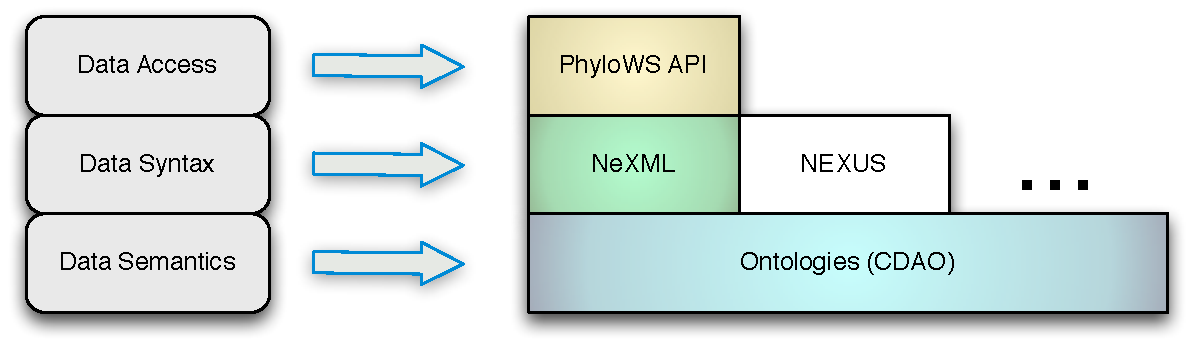
\includegraphics[width=0.6\textwidth]{EvoioStack.pdf}}
\caption{The EvoIO Stack}
\label{stack}
\end{figure}

\newpage

\subsection*{Figure 2 - The Principle View of OTUs and Characters}
This figure summarizes the core concepts from phylogenetic analysis that
are captured by the CDAO ontology.

\begin{figure}[h]
\centerline{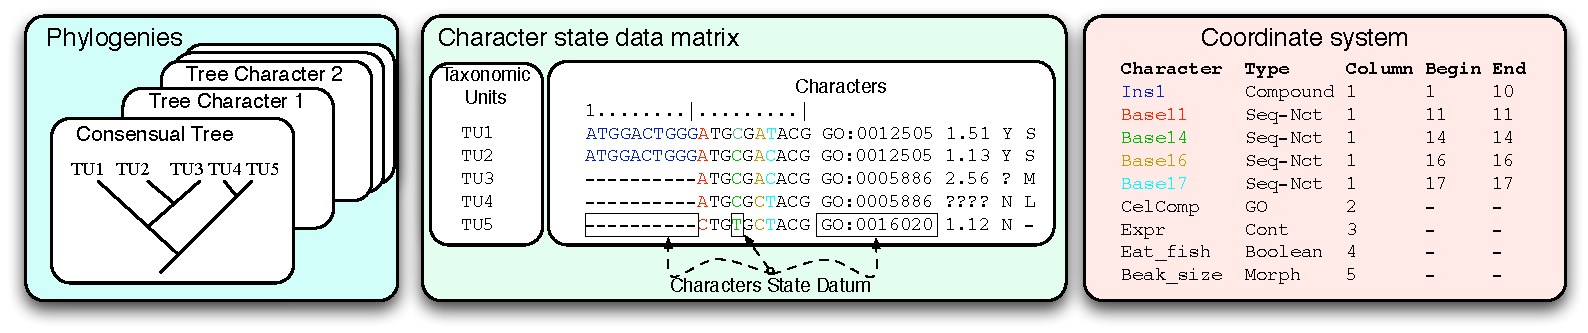
\includegraphics[width=0.9\textwidth]{cdofig.pdf}}
\caption{OTUs and Characters}
\label{cdao1}
\end{figure}

\newpage

\subsection*{Figure 3 - Snapshot of the Key concepts of CDAO}
This figure provides a very small summary of the core concepts and relations
described in CDAO.

\begin{figure}[h]
\centerline{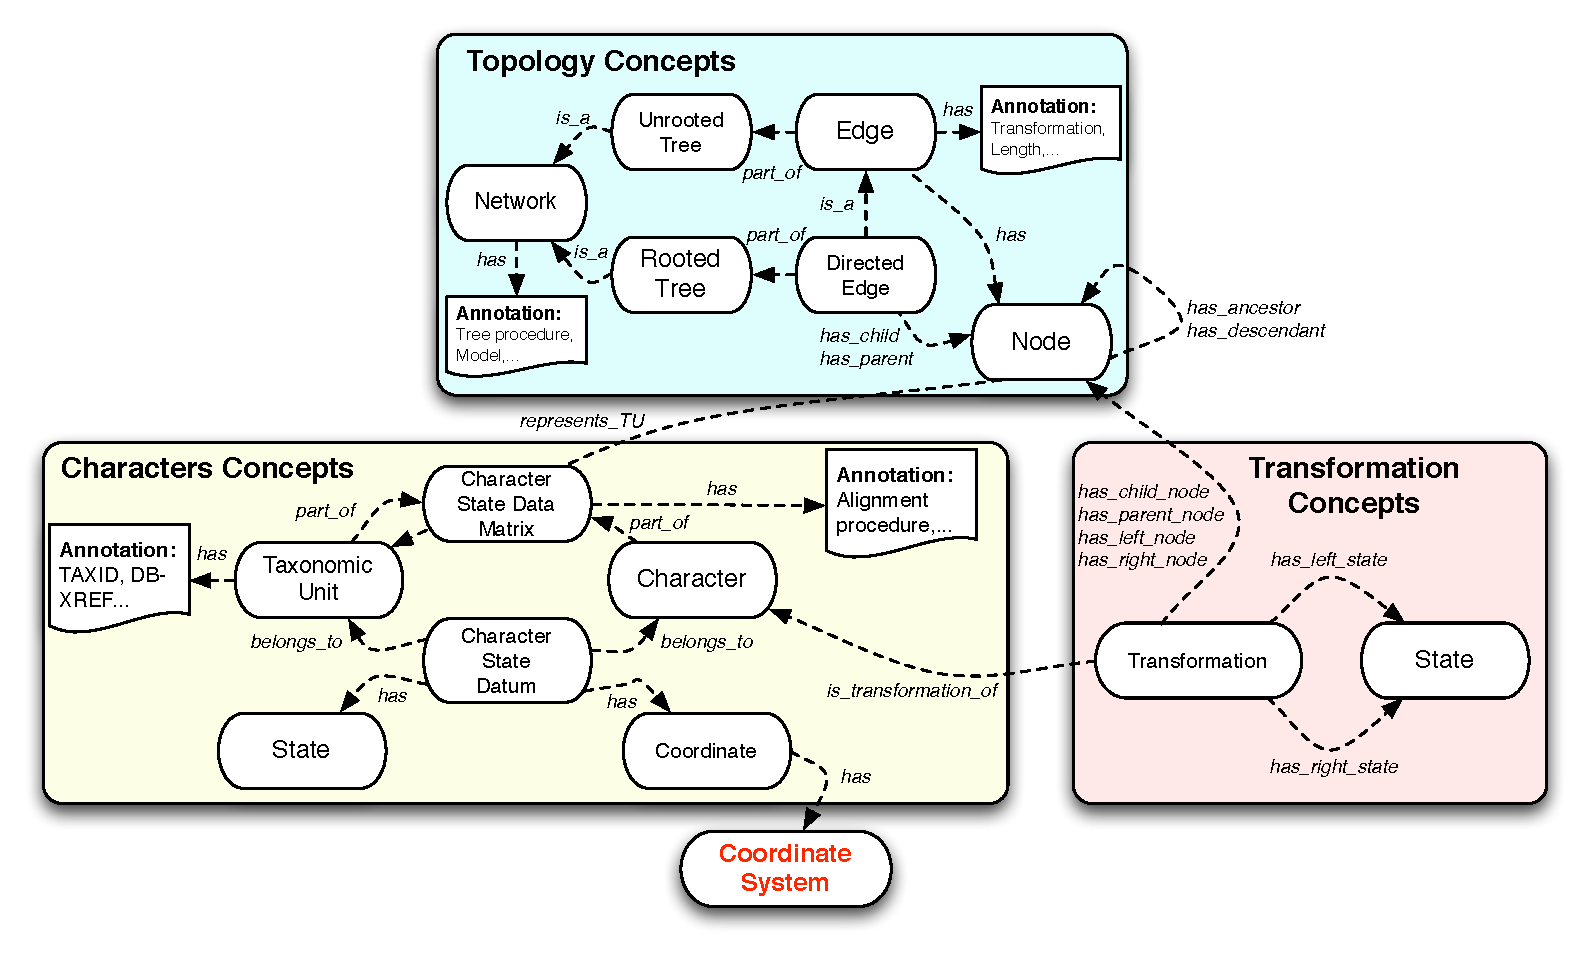
\includegraphics[width=0.8\textwidth]{cdao2.pdf}}
\caption{Core Concepts in CDAO}
\label{cdao2}
\end{figure}

\newpage

\subsection*{Figure 4 - Structure of CDAO-store}
This figure shows the overall structure of the implementation of the
CDAO-store.

\begin{figure}[h]
\centerline{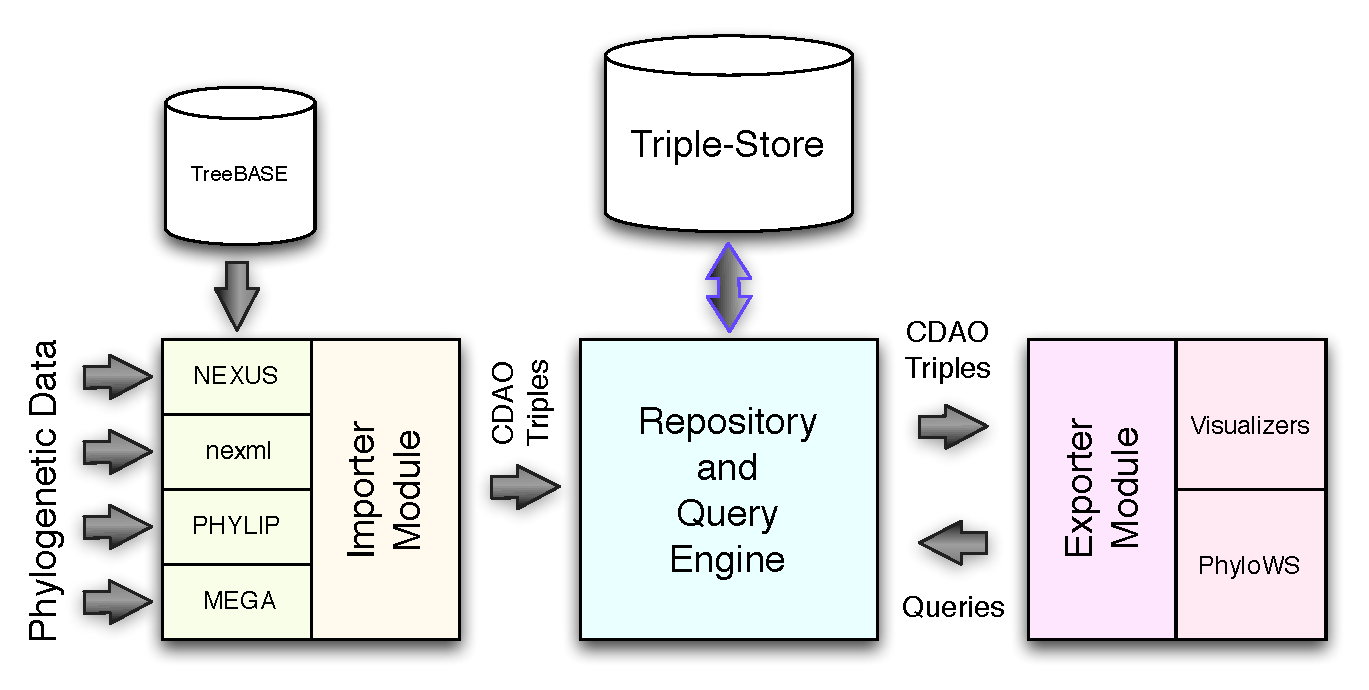
\includegraphics[width=0.9\textwidth]{struct.pdf}}
\caption{Overall Organization of CDAO-store}
\label{struct}
\end{figure}

\newpage

  \subsection*{Figure 5 - Tree Viewer with search}
This is the TreeViewer Application displaying the tree Tree3099 from TreeBase and searching for all nodes and edges with \verb|#Ilex_|.
      
\begin{figure}[h]
\centerline{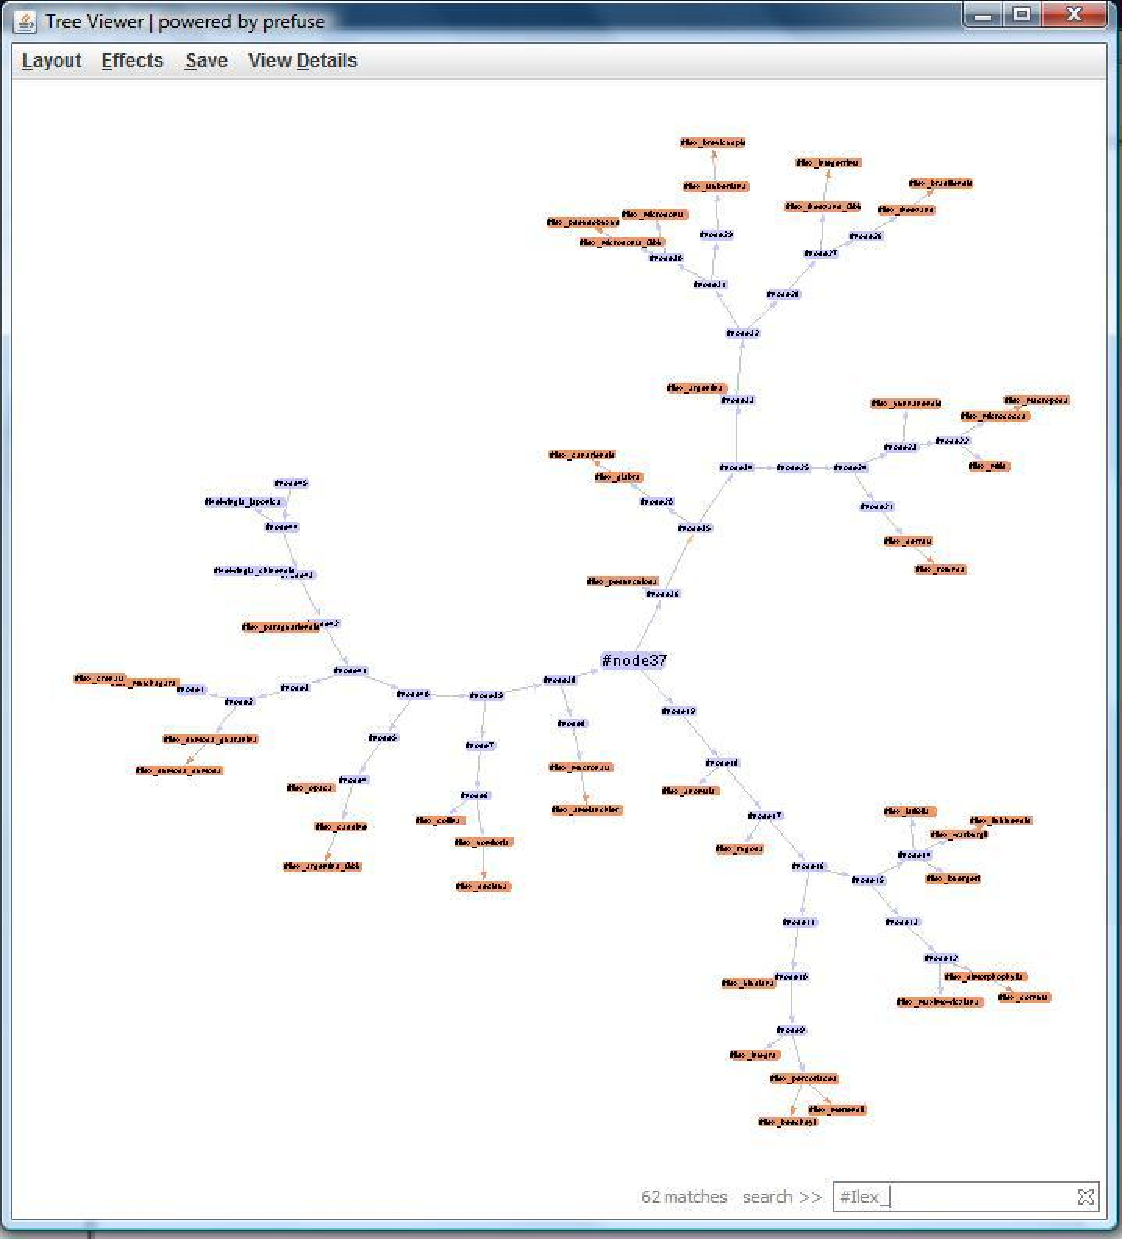
\includegraphics[width=0.8\textwidth]{TreeViewerSearch.pdf}}
\centerline{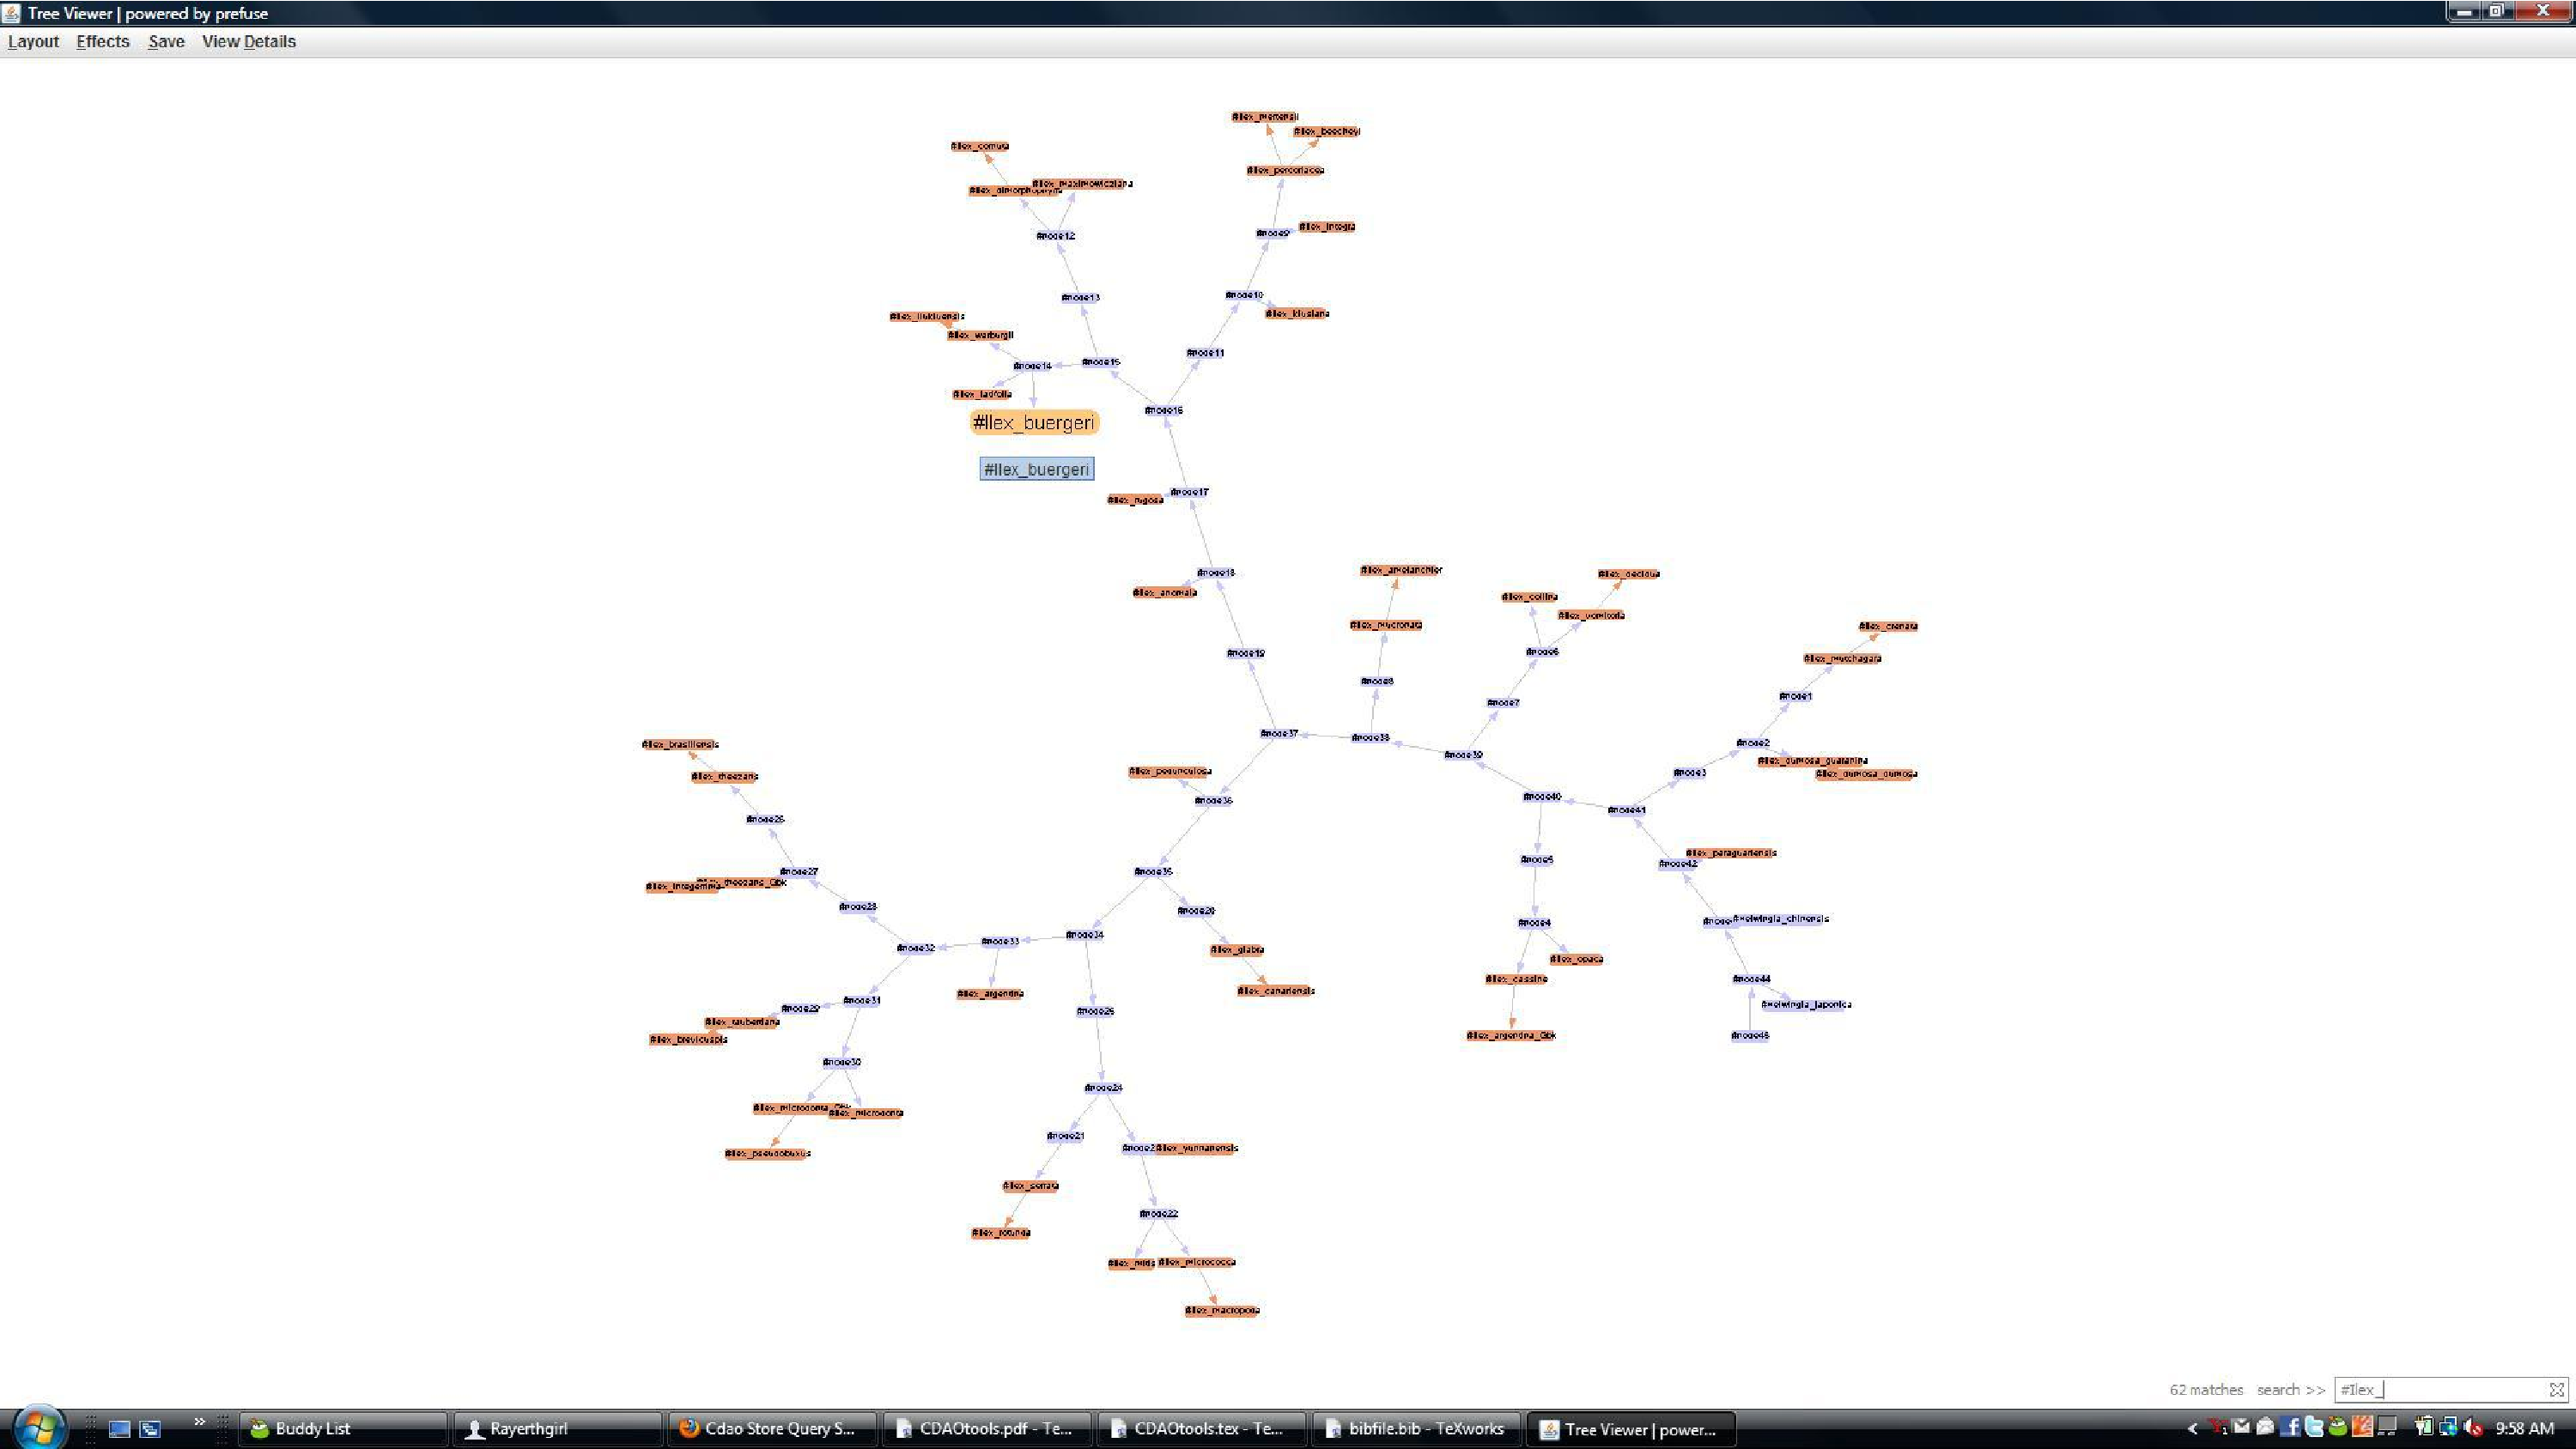
\includegraphics[width=0.8\textwidth]{TreeViewer_Search.pdf}}
\caption{TreeViewer Application with the force layout and the search feature.}
\label{treeview}
\end{figure}

\newpage

 \subsection*{Figure 6 - Matrix Viewer}

\begin{figure}[h]
\centerline{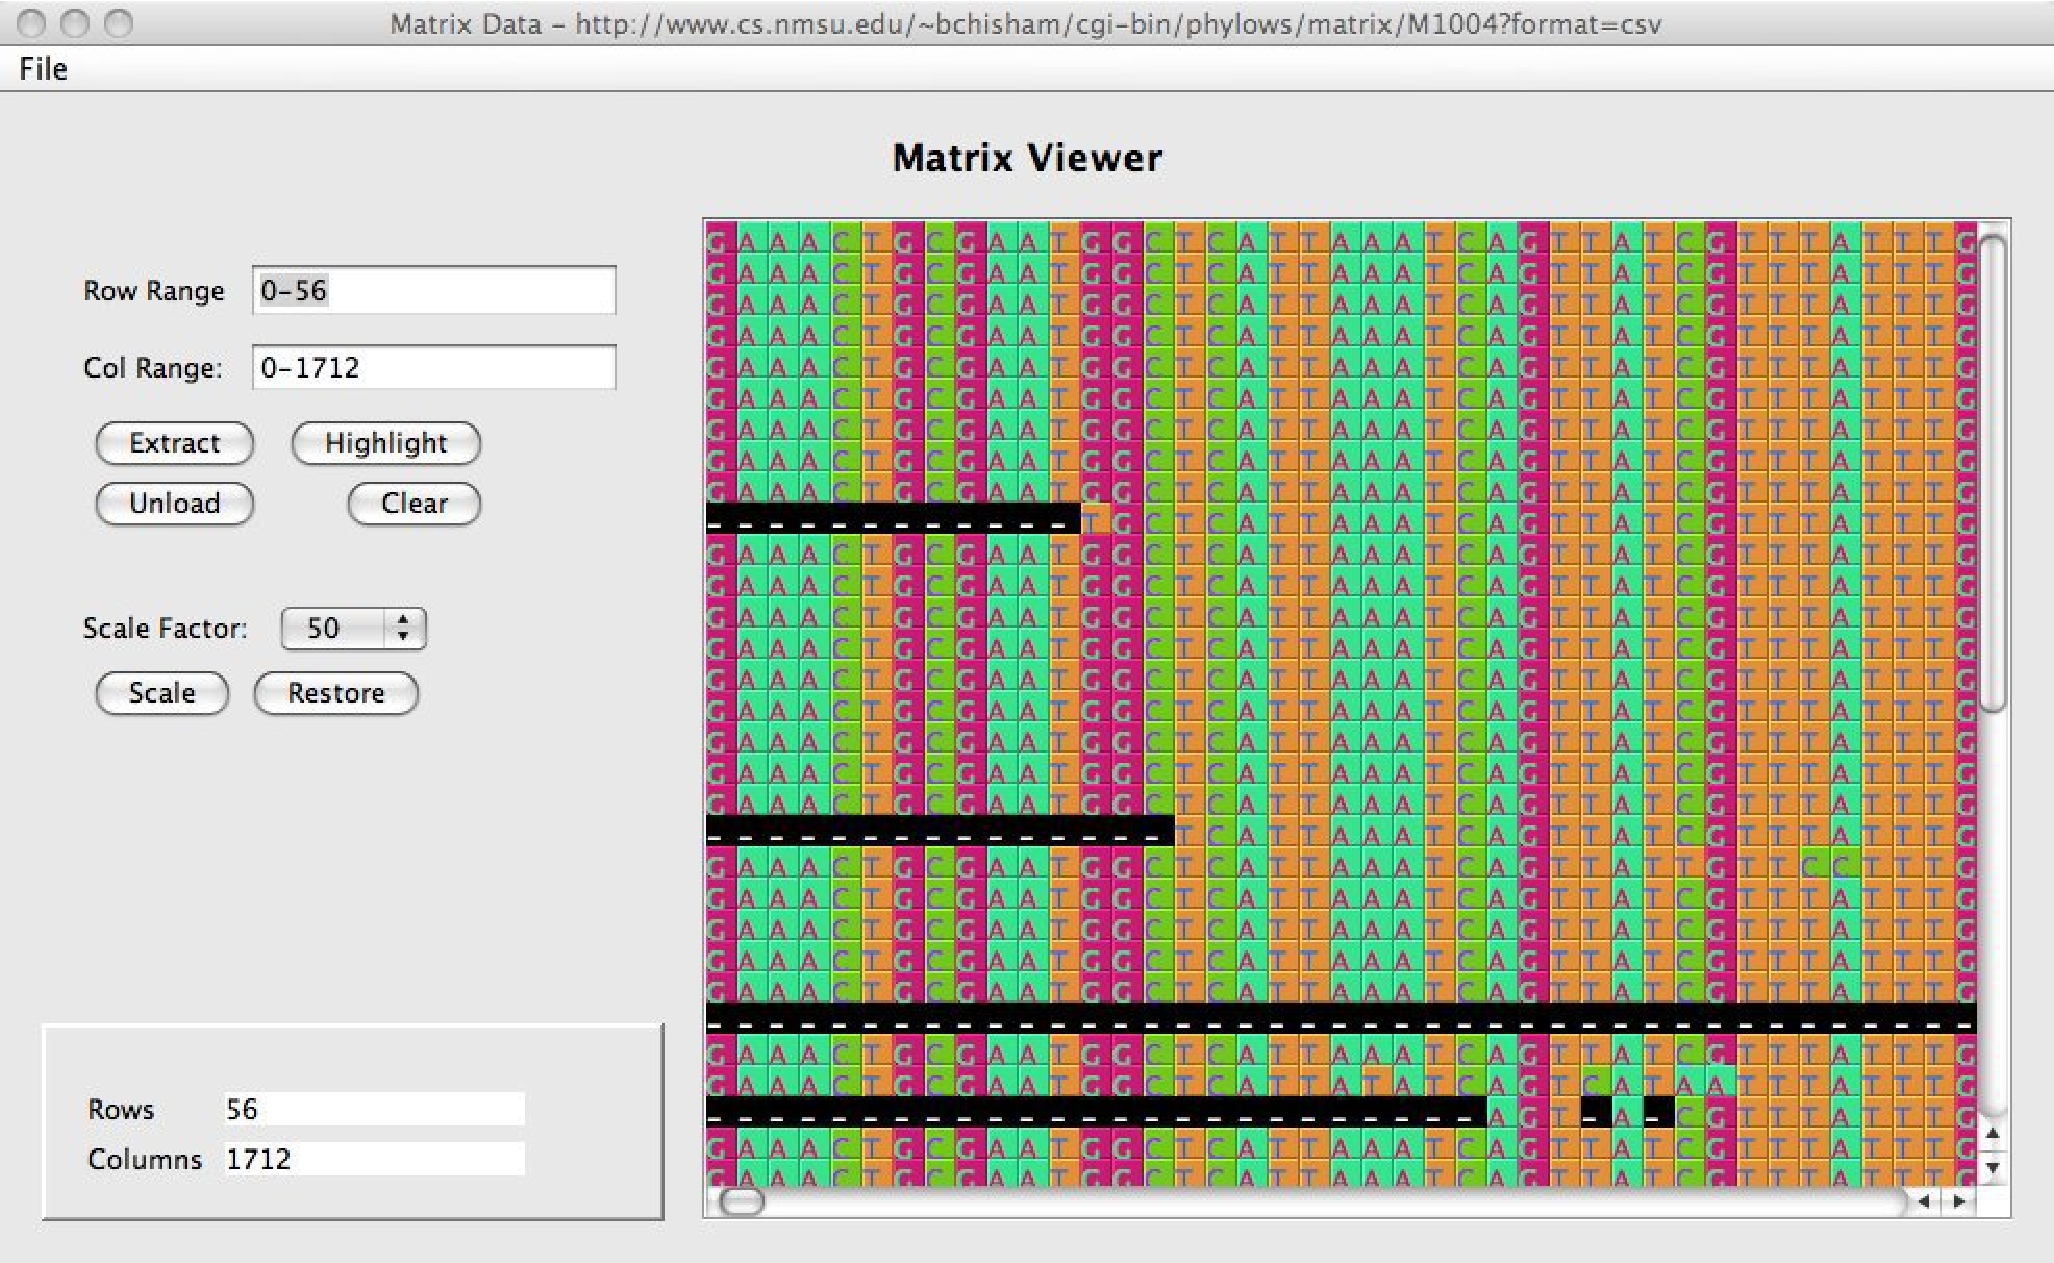
\includegraphics[width=0.8\textwidth]{matrix-view-m1004.pdf}}
\caption{MatrixViewer Application}
\label{matrix}
\end{figure} 


%  \subsection*{Figure 2 - Sample figure title}
%      Figure legend text.



%%%%%%%%%%%%%%%%%%%%%%%%%%%%%%%%%%%
%%                               %%
%% Tables                        %%
%%                               %%
%%%%%%%%%%%%%%%%%%%%%%%%%%%%%%%%%%%

%% Use of \listoftables is discouraged.
%%
%\section*{Tables}
%  \subsection*{Table 1 - Sample table title}
%    Here is an example of a \emph{small} table in \LaTeX\ using  
%    \verb|\tabular{...}|. This is where the description of the table 
%    should go. \par \mbox{}
%    \par
%    \mbox{
%      \begin{tabular}{|c|c|c|}
%        \hline \multicolumn{3}{|c|}{My Table}\\ \hline
%        A1 & B2  & C3 \\ \hline
   %     A2 & ... & .. \\ \hline
  %      A3 & ..  & .  \\ \hline
 %     \end{tabular}
%      }
%  \subsection*{Table 2 - Sample table title}
%    Large tables are attached as separate files but should
%    still be described here.



%%%%%%%%%%%%%%%%%%%%%%%%%%%%%%%%%%%
%%                               %%
%% Additional Files              %%
%%                               %%
%%%%%%%%%%%%%%%%%%%%%%%%%%%%%%%%%%%

\end{bmcformat}
\end{document}







